\chapter{Introduction}
\label{chap:intro}

Almost all modern SMT systems are trained using a large collection of translated
sentence pairs known as a parallel corpus. Sources of parallel data include
parliament proceedings, books, and news articles.
While this data may be abundant for some language pairs, such as
French/English, it is scarce for most others. In addition, even when parallel
data is available, it may not match the domain of the data you wish to
translate, and this can have a large effect on performance \citep{Munteanu05}.

The creation of new parallel corpora can be expensive, especially when bilingual
speakers are rare for the language pair of interest.
In order to acquire more parallel data without costly human annotation,
researchers have looked to corpora which may contain some parallel sentences,
but are not completely parallel. Such corpora are referred to as comparable
corpora, and examples include multilingual news feeds \citep{Munteanu05} and
Wikipedia articles \citep{Adafre06,Smith10}. 
Most work in extracting parallel sentences from
these corpora assumes an initial bilingual dictionary or an existing parallel
corpus.

On the other hand, there has also been work on aligning sentences in parallel
corpora where the documents may contain $2:1$ or $1:2$ sentence alignments, or
there may be large insertions or deletions of sentences \citep{Gale93,Chen93,Moore02}.
This work, by contrast, does not require existing parallel data or a
bilingual dictionary for the language pair of interest. Instead, the structure
of the documents and the lengths of the sentences are used to determine the
sentence alignment. Any information about bilingual word correspondence comes
from the parallel data that is being aligned.

In this work, we aim to combine techniques from both parallel and comparable
sentence alignment to improve the state of the art for parallel sentence
extraction from comparable corpora. First, we will describe a novel
discriminative model for aligning sentences in comparable documents.
We will also describe a model for aligning comparable documents which
needs only a minimal amount of supervision. Similar to how unsupervised word
alignment models can learn their parameters from unlabeled data, we aim to learn
parameters for a sentence alignment model from comparable unaligned documents.


\section{Sentence Alignment}
In this section, we will describe our task and notation.
We will view both parallel corpora alignment and the extraction of parallel
sentences from comparable corpora as an alignment task. In either type of
alignment we are given a set of bilingual document pairs in {\em source} and {\em
target} languages. When performing parallel corpora alignment, these document
pairs will correspond to each other very strongly, while in the case of
comparable corpora, some these document pairs may contain no parallel sentences.
\citet{Munteanu05} take their document pairs from news stories published at
roughly the same time, while \citet{Adafre06,Smith10} use entries from
Wikipedia that are on the same topic (Figure \ref{fig:wiki} gives and example).
The task of finding comparable document pairs is not addressed in this work.

\begin{figure*}[ht]
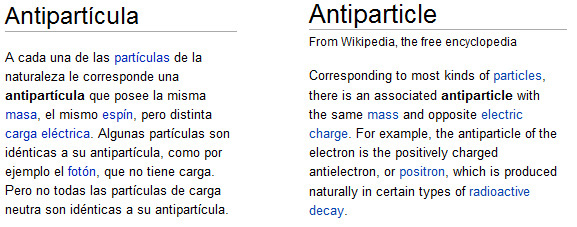
\includegraphics[width=\textwidth]{images/wiki.jpg}
\caption{An example of a Spanish/English document pair from Wikipedia.}
\label{fig:wiki}
\end{figure*}

Each document pair contains a sequence of source sentences (denoted by ${\bf
S}$) and target sentences (denoted by ${\bf T}$). Individual source and target
sentences are referred to by $S$ and $T$ respectively. Similarly, we refer to
the words within source and target sentences with the lowercase $s$ and $t$. We
borrow the notation of \citep{Och03} for describing alignments between sentences
as subsets of the Cartesian product of sentence positions. Sentence alignments
are referred to with the uppercase $A$, and word alignments with the lowercase
$a$.

The goal of sentence alignment is to identify which sentence pairs in the
bilingual document pairs are parallel. We view this as a retrieval task for
parallel sentence pairs, and so when annotated sentence alignments are present,
we can compute precision, recall, and F-measure.
